\documentclass[11pt, a4paper]{article}

% Paquetes básicos
\usepackage[utf8]{inputenc}
\usepackage[spanish]{babel}
\usepackage{amsmath}
\usepackage{graphicx}
\usepackage{booktabs}
\usepackage{geometry}
\usepackage{hyperref}
\usepackage{float}
\usepackage{cite}

\geometry{top=2.5cm, bottom=2.5cm, left=3cm, right=3cm}

\title{\textbf{Nota Técnica: Análisis de Deflexión en Viga Simplemente Apoyada}}
\author{Lucas Tejo Garrido \\\small Departamento de Ingeniería Civil en Obras Civiles, Universidad de Santiago de Chile.} 
\date{\today}

\begin{document}

\maketitle

\section{Problema y Objetivo}
El diseño y análisis de elementos estructurales requiere modelos matemáticos que predigan su comportamiento bajo carga, con el fin de verificar que los datos medidos son correctos o cercanos a la teoría. El objetivo de este documento es configurar un flujo de análisis reproducible para evaluar la respuesta elástica de una viga de sección rectangular simplemente apoyada y sometida a una carga puntual centrada. Se busca comparar un conjunto de datos medidos de carga-deflexión con las predicciones del modelo teórico lineal elástico de Euler-Bernoulli.

\section{Datos y Supuestos}
Para el análisis, se dispone de un conjunto de datos medidos de carga aplicada ($P$) en kN y la deflexión medida en el centro de la luz en mm. Los parámetros geométricos y elasticidad de la viga son:
\begin{itemize}
    \item Luz entre apoyos ($L$): $4\text{ m}$
    \item Ancho de la sección ($b$): $0.2\text{ m}$
    \item Altura de la sección ($h$): $0.4\text{ m}$
    \item Módulo de elasticidad ($E$): $25\text{ GPa}$
\end{itemize}
El análisis supone que el material es isotrópico. 

\section{Método}
El primer paso consistió en calcular el segundo momento de área ($I$) para una sección rectangular:
\begin{equation}
    I = \frac{b h^3}{12} = \frac{0.2 \cdot 0.4^3}{12} = 0.001067\text{ m}^4
\end{equation}

Luego, la deflexión teórica ($\delta_{teo}$) en el centro de la luz bajo una carga puntual $P$ se calcula mediante:
\begin{equation}
    \delta_{teo} = \frac{P L^3}{48 E I}
\end{equation}
Para asegurar la consistencia dimensional con la carga en kN y la geometría en metros, el módulo de elasticidad se transformó de GPa a $\text{kN/m}^2$, resultando en $E = 25 \times 10^6 \text{ kN/m}^2$. Finalmente, el resultado teórico en metros se multiplicó por $1000$ para su comparación en milímetros con los datos medidos. 

Para llevar acabo una comparación entre los resultados obtenidos teóricos y medidos, se utilizó la diferencia relativa:
\begin{equation}
    \text{Diferencia Relativa (\%)} = \left| \frac{\delta_{medida} - \delta_{teo}}{\delta_{teo}} \right| \times 100
\end{equation}

\section{Resultados y Verificación}
Mediante el uso de las formulas (2) y (3) para un intervalo de [5-40] para una carga $P$ se realizo la siguiente tabla de datos:

\begin{table}[H]
\centering
\caption{Comparación de carga, deflexión medida, deflexión teórica y diferencias.}
\label{tab:deflexion_viga}
\begin{tabular}{ccccc}
\toprule
\textbf{Carga [kN]} & \textbf{Deflexión [mm]} & \textbf{\shortstack{Deflexión\\ teórica [mm]}} & \textbf{\shortstack{Diferencia de\\ deflexión [mm]}} & \textbf{\shortstack{Diferencia\\ relativa [\%]}} \\ \midrule
0  & 0,00 & 0,00 & 0,00 & 0\% \\
5  & 0,26 & 0,25 & 0,01 & 4\% \\
10 & 0,50 & 0,50 & 0,00 & 0\% \\
15 & 0,76 & 0,75 & 0,01 & 1\% \\
20 & 1,01 & 1,00 & 0,01 & 1\% \\
25 & 1,28 & 1,25 & 0,03 & 2\% \\
30 & 1,54 & 1,50 & 0,04 & 3\% \\
35 & 1,77 & 1,75 & 0,02 & 1\% \\
40 & 2,05 & 2,00 & 0,05 & 3\% \\ \bottomrule
\end{tabular}
\end{table}

Luego, mediante análisis computacional se generó el gráfico de carga versus deflexión (Figura \ref{fig:carga_deflexion}), que superpone los datos medidos y el modelo teórico. La diferencia relativa calculada para cargas mayores a cero fluctuó en magnitudes muy pequeñas (entre 0\% y 4\%), demostrando una casi exacta similitud a lo calculado teóricamente.

\begin{figure}[H]
    \centering
    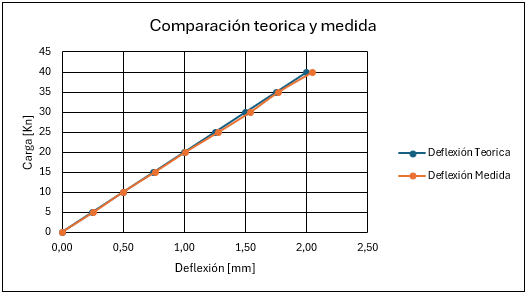
\includegraphics[width=0.7\textwidth]{carga_deflexion.png}
    \caption{Comparación entre deflexión medida y predicción de Euler-Bernoulli.}
    \label{fig:carga_deflexion}
\end{figure}

Como verificación adicional e independiente, se realizó un análisis dimensional explícito de la ecuación de deflexión para comprobar el resultado empírico:
\begin{equation}
    [\delta_{teo}] = \frac{[kN] \cdot [m]^3}{[kN/m^2] \cdot [m^4]} = \frac{kN \cdot m^3}{kN \cdot m^2} = [m]
\end{equation}
Finalmente, las conversiones de unidades realizadas para $E$ fueron consistentes y correctas.

\section{Interpretación y Conclusiones}
Los resultados indican que la teoría de Euler-Bernoulli es altamente precisa para predecir la deflexión en este caso de estudio dentro del rango de cargas evaluado (hasta 40 kN). La linealidad observada en los datos y la baja diferencia relativa confirman el comportamiento elástico del material. 

Una limitación directa del análisis es el uso de datos sintéticos ideales, los cuales no incluyen la variabilidad del material ni las imprecaciones de medición típicas de un ensayo de laboratorio real.

\section{Declaración de uso de IA}
\begin{itemize}
    \item \textbf{Herramienta:} Google Gemini 
    \item \textbf{Propósito del uso:} Apoyo en la estructuración de la nota técnica en LaTeX, elaboración de tablas y formulas.
    \item \textbf{Contenido incorporado:} Estructura base del código LaTeX (paquetes básicos) y códigos para la elaboración de tablas y fórmulas.
    \item \textbf{Verificación:} Todos los cálculos de inercia y transformación de unidades fueron comprobados manualmente paso a paso. La elaboración y desarrollo de los resultados de la tabla fueron realizados en hoja de calculo excel.
\end{itemize}

\cite{hibbeler2017}
\bibliographystyle{ieeetr}
\bibliography{referencias.bib}

\end{document}